\documentclass{article}

\usepackage{graphicx}
\usepackage{tikz}
\usepackage{tikzsymbols}
\usetikzlibrary{calc,patterns,shapes.geometric}
\pagestyle{empty}
\usepackage[margin=0pt]{geometry}
\geometry{papersize={14in,12in}}

\def\centerarc[#1](#2)(#3:#4:#5){\draw[#1] ($(#2)+({#5*cos(#3)},{#5*sin(#3)})$) arc (#3:#4:#5);}

\begin{document}
	\begin{figure}
		\centering
		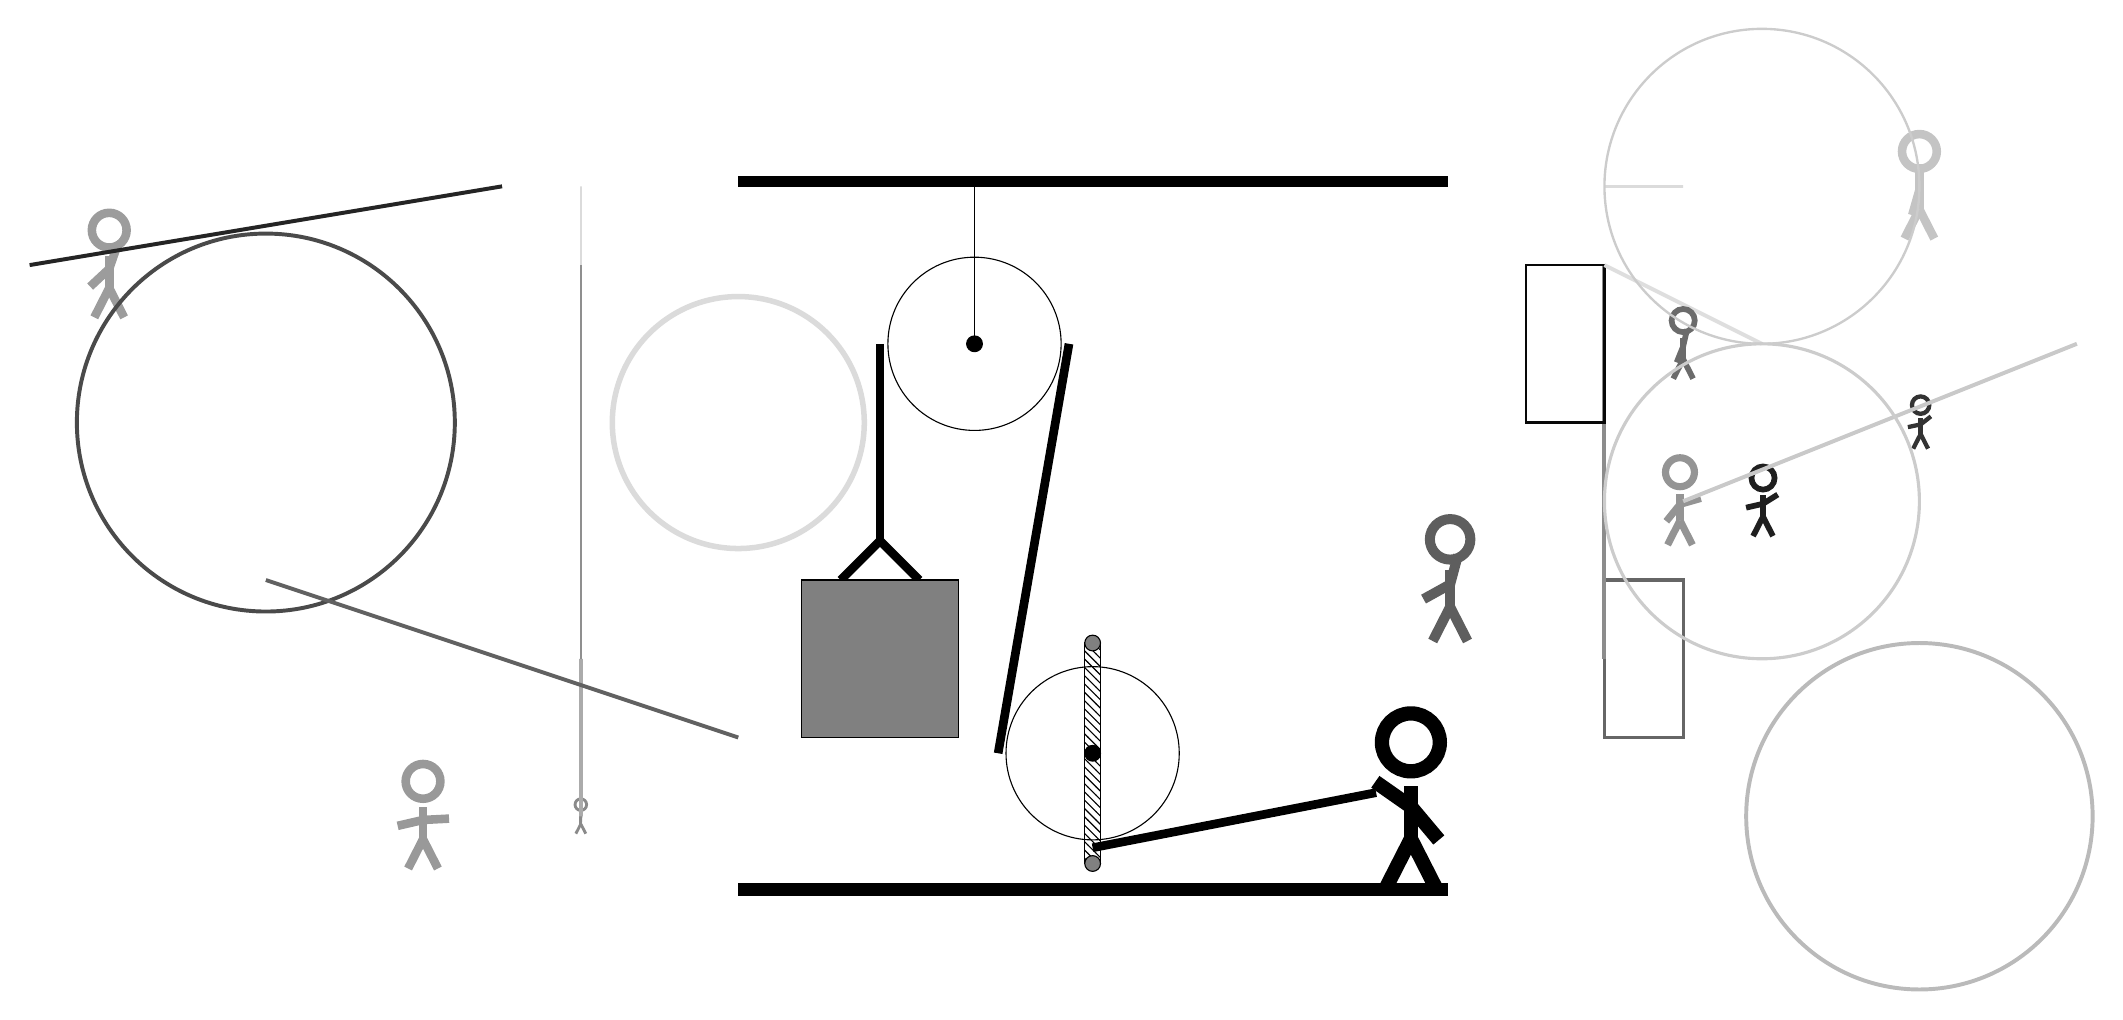
\begin{tikzpicture}
			%%%%% START %%%%%
			
			\draw[fill=black] (-2, 9) rectangle (7, 9.125);
			
			\draw (1, 7) circle (1.1);
			\draw[fill=black] (1, 7) circle (0.1);
			\draw (1, 9) -- (1, 7);
			
			\draw[fill=white](2.5, 1.8) circle (1.1);
			\draw[fill=black] (2.5, 1.8) circle (0.1);
			\draw[pattern=north west lines, pattern color=black] (2.4, 3.2) rectangle (2.6, 0.4);
			\draw[fill=black!50] (2.5, 3.2) circle (0.1);
			\draw[fill=black!50] (2.5, 0.4) circle (0.1);
			
			\draw[line width=1.1mm] (-0.7, 4.0) -- (-0.2, 4.5) -- (0.3, 4.0);
			\draw[fill=black!50] (-1.2, 4.0) rectangle (0.8, 2.0);
			
			\draw[line width=1.1mm] (-0.2, 7) -- (-0.2, 4.5);
			\centerarc[line width=1.1mm](1, 7)(0:180:1.2000000000000002);
			\draw[line width=1.1mm](2.2, 7) -- (1.3, 1.8);
			\centerarc[line width=1.1mm](2.5, 1.8)(180:270:1.2000000000000002);
			\draw[line width=1.1mm](2.5, 0.6) -- (6.1, 1.3);
			
			\draw[line width=0.4mm, color=black!60] (9, 2) rectangle (10, 4);
			
			\draw[line width=0.5mm, color=black!45] (9, 3) rectangle (9, 8);
			\node[line width=0.2mm, color=black!39] at (-10, 8) {\Strichmaxerl[6][43][71]};
			\draw[line width=0.3mm, color=black!97] (8, 6) rectangle (9, 8);
			\node[line width=0.7mm, color=black!46] at (-4, 1) {\Strichmaxerl[2][87][87]};
			
			\draw[line width=0.5mm, color=black!13](9, 8) -- (11, 7);
			\node[line width=0.6mm, color=black!23] at (13, 9) {\Strichmaxerl[6][74][90]};
			\draw[line width=0.5mm, color=black!86](-5, 9) -- (-11, 8);
			\draw [line width=0.7mm, color=black!14](-2, 6) circle (1.6);
			
			\draw [line width=0.5mm, color=black!27](13, 1) circle (2.2);
			
			\node[line width=0.4mm, color=black!58] at (10, 7) {\Strichmaxerl[4][68][77]};
			\draw[line width=0.2mm, color=black!14] (-4, 9) rectangle (-4, 8);
			\node[line width=0.2mm, color=black!40] at (-6, 1) {\Strichmaxerl[6][13][3]};
			
			\draw[line width=0.5mm, color=black!33] (-4, 1) rectangle (-4, 3);
			\node[line width=0.2mm, color=black!88] at (11, 5) {\Strichmaxerl[4][13][32]};
			\node[line width=0.2mm, color=black!80] at (13, 6) {\Strichmaxerl[3][12][38]};
			
			\node[line width=0.3mm, color=black!42] at (10, 5) {\Strichmaxerl[5][51][16]};
			
			\draw[line width=0.4mm, color=black!14] (9, 9) rectangle (10, 9);
			\draw [line width=0.5mm, color=black!71](-8, 6) circle (2.4);
			\draw[line width=0.5mm, color=black!21](10, 5) -- (15, 7);
			\draw [line width=0.4mm, color=black!20](11, 5) circle (2.0);
			
			\node[line width=0.4mm, color=black!63] at (7, 4) {\Strichmaxerl[7][29][75]};
			\draw [line width=0.3mm, color=black!20](11, 9) circle (2.0);
			\draw[line width=0.2mm, color=black!44] (-4, 8) rectangle (-4, 3);
			\draw[line width=0.5mm, color=black!62](-2, 2) -- (-8, 4);
			
			\node at (6.5, 1.2) {\Strichmaxerl[10][-35][-50]};
			
			\draw[fill=black] (-2, 0) rectangle (7, 0.15);
			
			%%%%% END %%%%%
		\end{tikzpicture}
	\end{figure}	
\end{document}